% !TEX TS-program = xelatex
% !BIB program = bibtex
% !TEX encoding = UTF-8 Unicode

\documentclass[
  twoside,
  openright,
  degree    = master,               % degree = master | doctor
  language  = english,              % language = chinese | english
  fontset   = template,             % fontset = default | template | system | overleaf
  watermark = true,                 % watermark = true | false
  doi       = true,                 % doi = true | false
]{ntuthesis}

% !TeX root = ./main.tex

% --------------------------------------------------
% 資訊設定(Information Configs)
% --------------------------------------------------

\ntusetup{
  university*   = {National Taiwan University},
  university    = {國立臺灣大學},
  college       = {工學院},
  college*      = {College of Engineering},
  institute     = {工業工程學研究所},
  institute*    = {Department of Industrial Engineering}, % 請確認您的科系為Department of xxx或Institute of xxx
  title         = {國立臺灣大學碩博士畢業論文模版},
  title*        = {National Taiwan University (NTU) \\ Thesis/Dissertation Template in \LaTeX},
  author        = {彭新翔},
  author*       = {Hsin-Hsiang Peng},
  ID            = {R05546030},
  advisor       = {吳文方},
  advisor*      = {Wen-Fang Wu},
  date          = {2020-05-01},         % 若註解掉,則預設為當天
  oral-date     = {2020-05-01},         % 若註解掉,則預設為當天
  DOI           = {10.5566/NTU2018XXXXX},
  keywords      = {LaTeX, 中文, 論文, 模板},
  keywords*     = {LaTeX, CJK, Thesis, Template},
}

% --------------------------------------------------
% 加載套件(Include Packages)
% --------------------------------------------------

\usepackage[sort&compress]{natbib}      % 參考文獻
\usepackage{amsmath, amsthm, amssymb}   % 數學環境
\usepackage{ulem, CJKulem}              % 下劃線、雙下劃線與波浪紋效果
\usepackage{booktabs}                   % 改善表格設置
\usepackage{multirow}                   % 合併儲存格
\usepackage{diagbox}                    % 插入表格反斜線
\usepackage{array}                      % 調整表格高度
\usepackage{longtable}                  % 支援跨頁長表格
\usepackage{paralist}                   % 列表環境
\usepackage{tabularx}  % auto-wrapping column type X
\usepackage{makecell}



\usepackage{lipsum}                     % 英文亂字
\usepackage{zhlipsum}                   % 中文亂字

% --------------------------------------------------
% 套件設定(Packages Settings)
% --------------------------------------------------
\setlength\tabcolsep{3pt}       % tighter column padding
\newcolumntype{L}[1]{>{\raggedright\arraybackslash}p{#1}}

\begin{document}

% 封面與口試審定
% Cover and Verification Letter
\makecover                          % 論文封面(Cover)
\makeverification                   % 口試委員審定書(Verification Letter)

% 致謝與論文摘要
% Acknowledgement and Abstract
% \pagenumbering{roman}             % 若您隱藏口委審定書 請解開此註解 頁碼會從致謝開始(羅馬數字)
\input{front/acknowledgement}       % 致謝(Acknowledgement)
\input{front/abstract}              % 摘要(Abstract)

% 生成目錄與符號列表
% Contents of Tables and Denotation
\maketableofcontents                % 目錄(Table of Contents)
\makelistoffigures                  % 圖目錄(List of Figures)
\makelistoftables                   % 表目錄(List of Tables)
\input{front/denotation}            % 符號列表(Denotation)

% 論文內容
% Contents of Thesis
\mainmatter
% !TeX root = ../main.tex

\chapter{Introduction}

This chapter introduces the research background and motivation.


% !TeX root = ../main.tex

\chapter{Literature}

This chapter reviews related literature and theoretical background.


% !TeX root = ../main.tex

\chapter{Data \& Dictionary Construction}

This chapter describes the data sources and dictionary creation process.

\begin{table}[htbp]
\centering
\caption{Table 1: Search Query for the Taiwan Cross-Strait GPR Index}
\begin{tabular}{llll}
\toprule
Category & Search query & Peak (week) & Contribution to index percent \\
\midrule
\multicolumn{4}{l}{\textbf{Panel A. Search categories and search queries}} \\
Military Escalation & military\_threats AND cross\_strait\_relations & & \\
Foreign Intervention Risk & foreign\_intervention AND military\_threats & & \\
Economic Coercion & economic\_coercion AND cross\_strait\_relations & & \\
Cyber and Information Warfare & cyber\_and\_information\_warfare AND cross\_strait\_relations & & \\
Diplomatic Crisis & diplomatic\_incidents AND foreign\_intervention & & \\
Internal Political Instability & internal\_political\_risk AND cross\_strait\_relations & & \\
Critical Infrastructure Threat & critical\_infrastructure\_threats AND military\_threats & & \\
\midrule
\multicolumn{4}{l}{\textbf{Panel B. Search word sets}} \\
\textit{military\_threats} &
\multicolumn{3}{l}{%
\begin{tabular}[t]{@{}l@{}}
軍事威脅, 武力犯台, 軍演, 軍事演習, 共軍, 解放軍, 軍機擾台, 軍艦繞台,\\
飛彈試射, 戰備警戒, 防空識別區, 空中攔截, 軍事衝突, 台海危機, 軍事部署, 戰爭邊緣
\end{tabular}
} \\
\textit{cross\_strait\_relations} &
\multicolumn{3}{l}{%
\begin{tabular}[t]{@{}l@{}}
兩岸關係, 台海局勢, 台海緊張, 和平協議, 九二共識, 一國兩制, 統一, 分裂, 台獨,\\
獨立公投, 和平發展, 敵對狀態, 兩岸對話, 兩岸交流
\end{tabular}
} \\
\textit{foreign\_intervention} &
\multicolumn{3}{l}{%
\begin{tabular}[t]{@{}l@{}}
美國介入, 美台關係, 美國軍售, 美國國會訪台, 美國支持, 日台合作, 日美安保,\\
國際聲援, 外國干預, 外國勢力, 國際制裁, 聯合國, 外交承認, 邦交國
\end{tabular}
} \\
\textit{economic\_coercion} &
\multicolumn{3}{l}{%
\begin{tabular}[t]{@{}l@{}}
經濟制裁, 貿易封鎖, 禁運, 斷交, 出口限制, 進口禁令, 經濟脅迫,\\
產業鏈轉移, 投資審查, 金融制裁, 資本外流, 供應鏈中斷
\end{tabular}
} \\
\textit{cyber\_and\_information\_warfare} &
\multicolumn{3}{l}{%
\begin{tabular}[t]{@{}l@{}}
網路攻擊, 駭客入侵, 資訊戰, 假消息, 認知作戰, 網軍, 輿論操控,\\
網路滲透, 資安威脅, 假新聞, 網路戰爭
\end{tabular}
} \\
\textit{diplomatic\_incidents} &
\multicolumn{3}{l}{%
\begin{tabular}[t]{@{}l@{}}
外交衝突, 召回大使, 抗議, 譴責, 外交斷交, 外交壓力, 國際孤立,\\
外交爭端, 外交抗議, 外交危機
\end{tabular}
} \\
\textit{internal\_political\_risk} &
\multicolumn{3}{l}{%
\begin{tabular}[t]{@{}l@{}}
政黨輪替, 總統大選, 罷免, 立法院衝突, 社會動盪, 抗議活動,\\
群眾運動, 政治分歧, 內部矛盾, 政變, 政局不穩
\end{tabular}
} \\
\textit{critical\_infrastructure\_threats} &
\multicolumn{3}{l}{%
\begin{tabular}[t]{@{}l@{}}
關鍵基礎設施, 電力中斷, 通訊癱瘓, 能源危機, 交通癱瘓, 水資源短缺,\\
基礎設施攻擊, 供電中斷, 網路癱瘓
\end{tabular}
} \\
\bottomrule
\end{tabular}
\end{table}

The language model dictionary captures a much broader set of hybrid warfare
concepts than the manually crafted dictionary. Six of the seven categories do
not belong to traditional warfare risks. This difference indicates that the
model reflects local and recent trends. Taiwan's objective is to deter a
possible invasion from China, while China seeks to counter such preparations.
Thus, terms related to economic coercion, potential foreign intervention,
diplomatic isolation, infrastructure threats, and cyber and information
attacks are relevant. Words describing direct war acts appear less frequently
because no large-scale conflict has occurred in decades, making a standard
global dictionary such as \citet{caldara2013geopoliticalrisk} less suitable.
The language model also yields a more balanced set of categories, with the top
contributor accounting for only 33\% compared with Lau's 86\%.


% !TeX root = ../main.tex

\chapter{GPR Index: Computation \& Time-Series Results}

This chapter details the computation of the GPR index and presents the time-series results.

\begin{figure}[htbp]
  \centering
  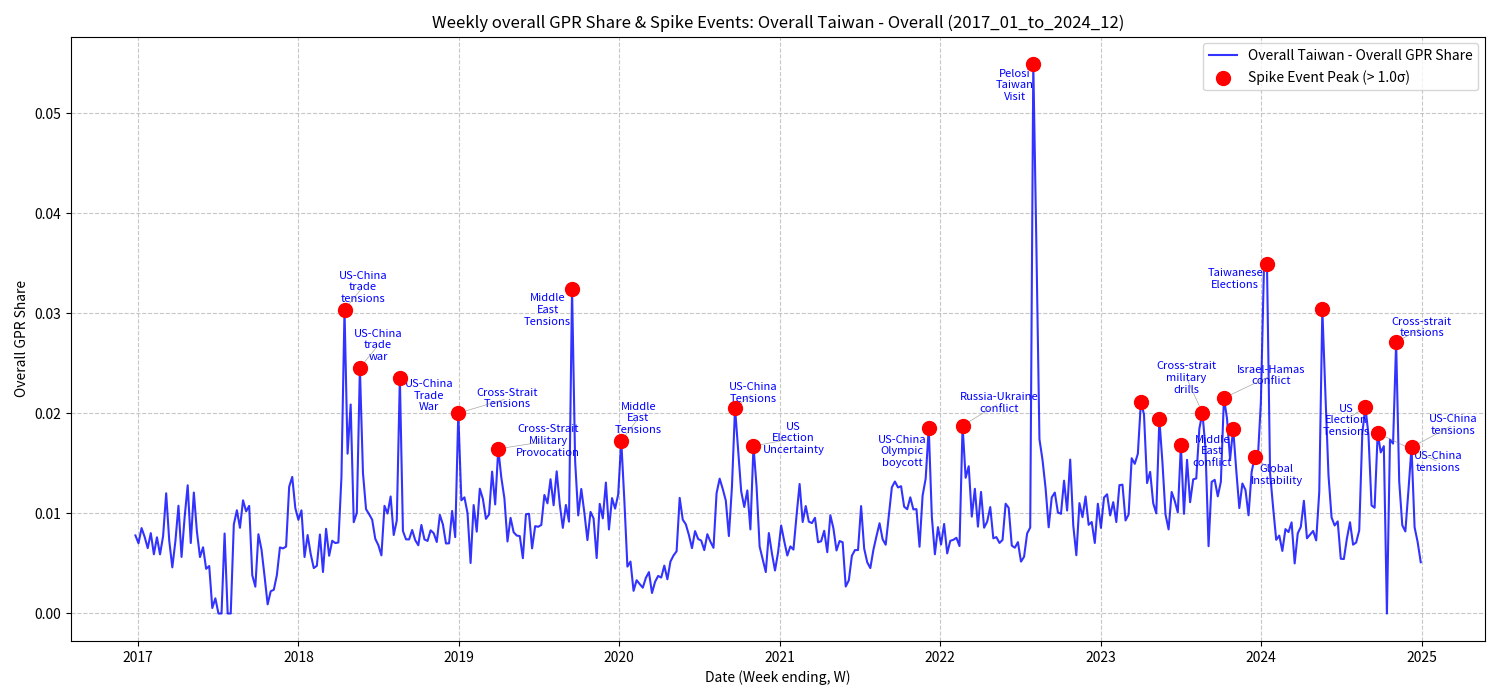
\includegraphics[width=\linewidth]{gpr_spike_events_llm_overall_Overall_Taiwan_2017_01_to_2024_12.png}
  \caption{Weekly GPR Index with LLM dictionary}
  \label{fig:my_example}
\end{figure}

\begin{figure}[htbp]
  \centering
  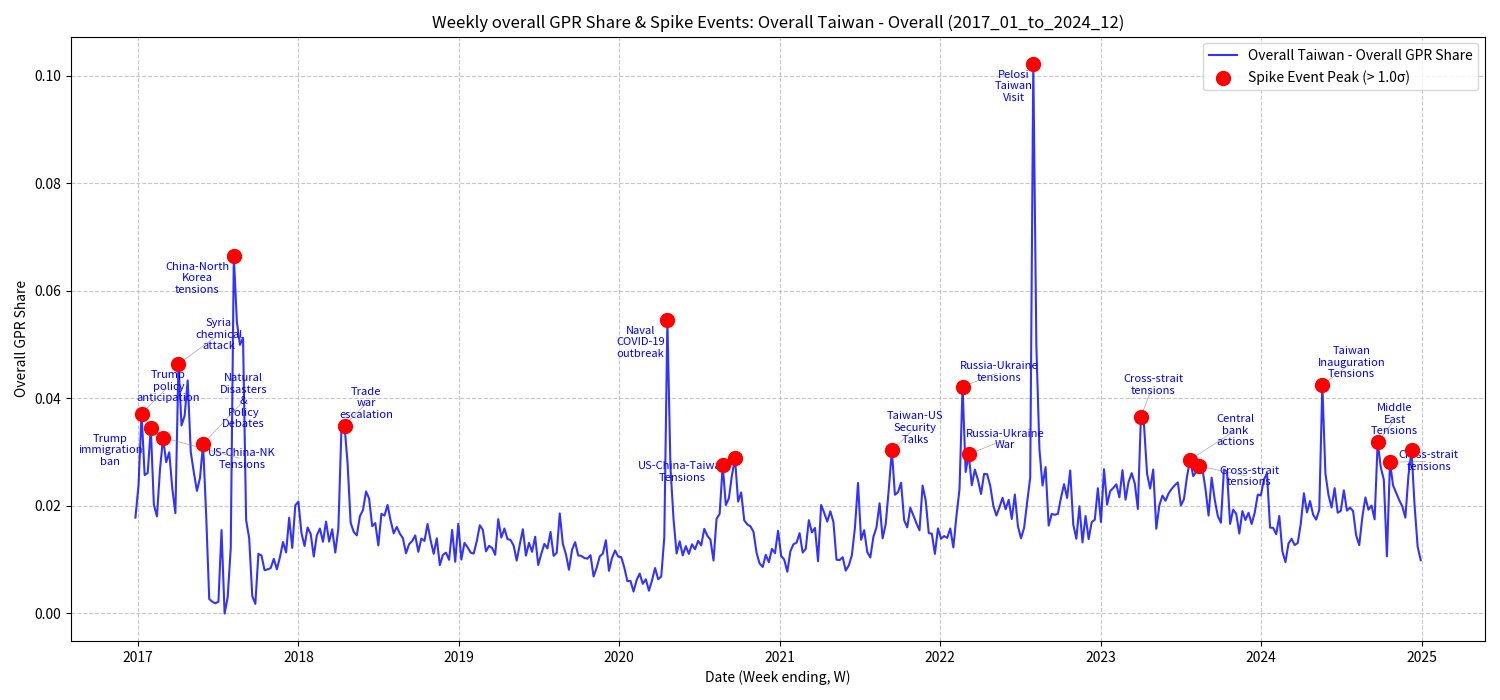
\includegraphics[width=\linewidth]{gpr_spike_events_llm_overall_Overall_Taiwan_2017_01_to_2024_12_lau.png}
  \caption{Weekly GPR Index with Lau's dictionary}
  \label{fig:my_example}
\end{figure}

% 參考文獻
% References
\refmatter
\bibliographystyle{abbrv}
\bibliography{back/references}

% 附錄
% Appendices
% !TeX root = ../main.tex

\appendix{A}{Five LLM Dictionaries}

This appendix lists the five language model dictionaries used in the analysis.


% !TeX root = ../main.tex

\appendix{B}{Supplementary Tables / Code Links}

This appendix provides supplementary tables and links to the code.



\end{document}
